\documentclass[12pt,a4paper]{article}
\usepackage{ctex}
\usepackage{amsmath,amssymb,amsfonts}
\usepackage{geometry}
\geometry{margin=2.5cm}
\usepackage{graphicx}
\graphicspath{{./}}
\usepackage{hyperref}
\hypersetup{colorlinks=true,linkcolor=blue,citecolor=blue,urlcolor=blue}
\usepackage{fancyhdr}
\pagestyle{fancy}
\fancyhead[L]{\small 量子场论入门}
\fancyhead[R]{\small DeepSeek}
\usepackage{setspace}
\onehalfspacing
\usepackage{enumitem}
\usepackage[bottom]{footmisc}

\title{\vspace{-2em}\textbf{量子场论入门}\\
\large 从谐振子到 Feynman 图——Phase 0--2：概念基础与数值实践}

\author{\texttt{DeepSeek}}
\date{2026 年 5 月}

\begin{document}
\maketitle
\vspace{-1em}

\section{引言}

这一节的目标只有一个：搞清楚\textbf{算符场} $\hat\phi(x)$ 到底是什么。
我们从你最熟悉的东西出发——简谐振子。

\section{单量子谐振子（QHO）}

你之前解过谐振子的波函数，这里我们从产生湮灭算符的角度来复习。

\subsection{算符代数}

一个质量为 $m=1$、频率为 $\omega$ 的谐振子：
\begin{equation}
\hat H = \frac{1}{2}\hat p^2 + \frac{1}{2}\omega^2 \hat x^2,
\qquad [\hat x, \hat p] = i.
\label{eq:qho-ham}
\end{equation}

定义产生湮灭算符：
\begin{equation}
\hat a = \sqrt{\frac{\omega}{2}}\left(\hat x + \frac{i}{\omega}\hat p\right),\qquad
\hat a^\dagger = \sqrt{\frac{\omega}{2}}\left(\hat x - \frac{i}{\omega}\hat p\right).
\label{eq:annihilation}
\end{equation}

它们满足：
\begin{equation}
[\hat a, \hat a^\dagger] = 1,
\qquad
\hat H = \omega\left(\hat a^\dagger \hat a + \frac12\right).
\label{eq:qho-comm}
\end{equation}

\subsection{粒子数表象}

基态 $|0\rangle$ 由 $\hat a|0\rangle = 0$ 定义。
激发态为
\begin{equation}
|n\rangle = \frac{(\hat a^\dagger)^n}{\sqrt{n!}}|0\rangle,
\qquad
\hat a^\dagger \hat a |n\rangle = n|n\rangle.
\label{eq:fock-state}
\end{equation}

这个 $|n\rangle$ 空间叫做\textbf{Fock 空间}——它是所有可能的激发数 $n$ 的张量积空间
\begin{equation}
\mathcal{F} = \bigoplus_{n=0}^\infty \mathcal{H}_n,
\label{eq:fock-space}
\end{equation}
其中 $\mathcal{H}_n$ 是 $n$ 粒子子空间。

这是 DMRG/MPS 的张量网络直觉可以直接对接的地方：
在 MPS 中，每个 site 有 $d$ 维 local Hilbert 空间 $\mathbb{C}^d$，
而谐振子相当于 $d = \infty$ 的 site。

\section{从谐振子到场}

\subsection{耦合谐振子链}

现在把 $N$ 个谐振子排成一维链，相邻之间用弹簧耦合：

\begin{equation}
\hat H = \sum_{i=1}^N \left[\frac{1}{2}\hat p_i^2 + \frac{1}{2}\omega_0^2 \hat x_i^2\right]
+ \frac{g}{2}\sum_{i=1}^{N-1} (\hat x_{i+1} - \hat x_i)^2.
\label{eq:chain-ham}
\end{equation}

其中第一项是每个 site 的 local 谐振子势，第二项是最近邻耦合。
这个 Hamiltonian 可以直接对角化：做离散傅里叶变换

\begin{equation}
\hat x_k = \frac{1}{\sqrt{N}}\sum_j \hat x_j e^{-ikj},
\qquad
\hat p_k = \frac{1}{\sqrt{N}}\sum_j \hat p_j e^{-ikj},
\label{eq:fourier}
\end{equation}

其中 $k = 2\pi n/N$（$n = 0, 1, \ldots, N-1$）。

对角化后的 Hamiltonian 是 $N$ 个\textbf{解耦的简正模式}：
\begin{equation}
\hat H = \sum_k \left[\frac{1}{2}|\hat p_k|^2 + \frac{1}{2}\omega_k^2 |\hat x_k|^2\right],
\label{eq:diag-ham}
\end{equation}
其中色散关系为
\begin{equation}
\omega_k^2 = \omega_0^2 + 4g\, \sin^2\frac{k}{2}.
\label{eq:dispersion}
\end{equation}

\textbf{核心结论：}每个简正模式 $k$ 是一个独立的谐振子，
可以用自己的产生湮灭算符 $a_k^\dagger, a_k$ 来描述。

\begin{equation}
\hat H = \sum_k \omega_k \left(a_k^\dagger a_k + \frac12\right).
\label{eq:diag-qho}
\end{equation}

以上推导可直接用 Python 数值验证。代码 \texttt{04\_coupled\_qho.py}\footnote{见 GitHub: \url{https://github.com/hy-wu/qft_coding}} 构建 $N$ 个耦合 QHO 的 Hamiltonian 矩阵，通过精确对角化得到本征频率 $\omega_k$。

图~\ref{fig:dispersion} 展示了 $N=32$ 个格点的色散关系。在长波极限 $k \ll \pi/a$ 下，数值结果精确趋近连续相对论色散 $\omega_k \approx \sqrt{\omega_0^2 + k^2}$（在最低非零模式处相对偏差仅 $0.12\%$）。

\begin{figure}[htbp]
\centering
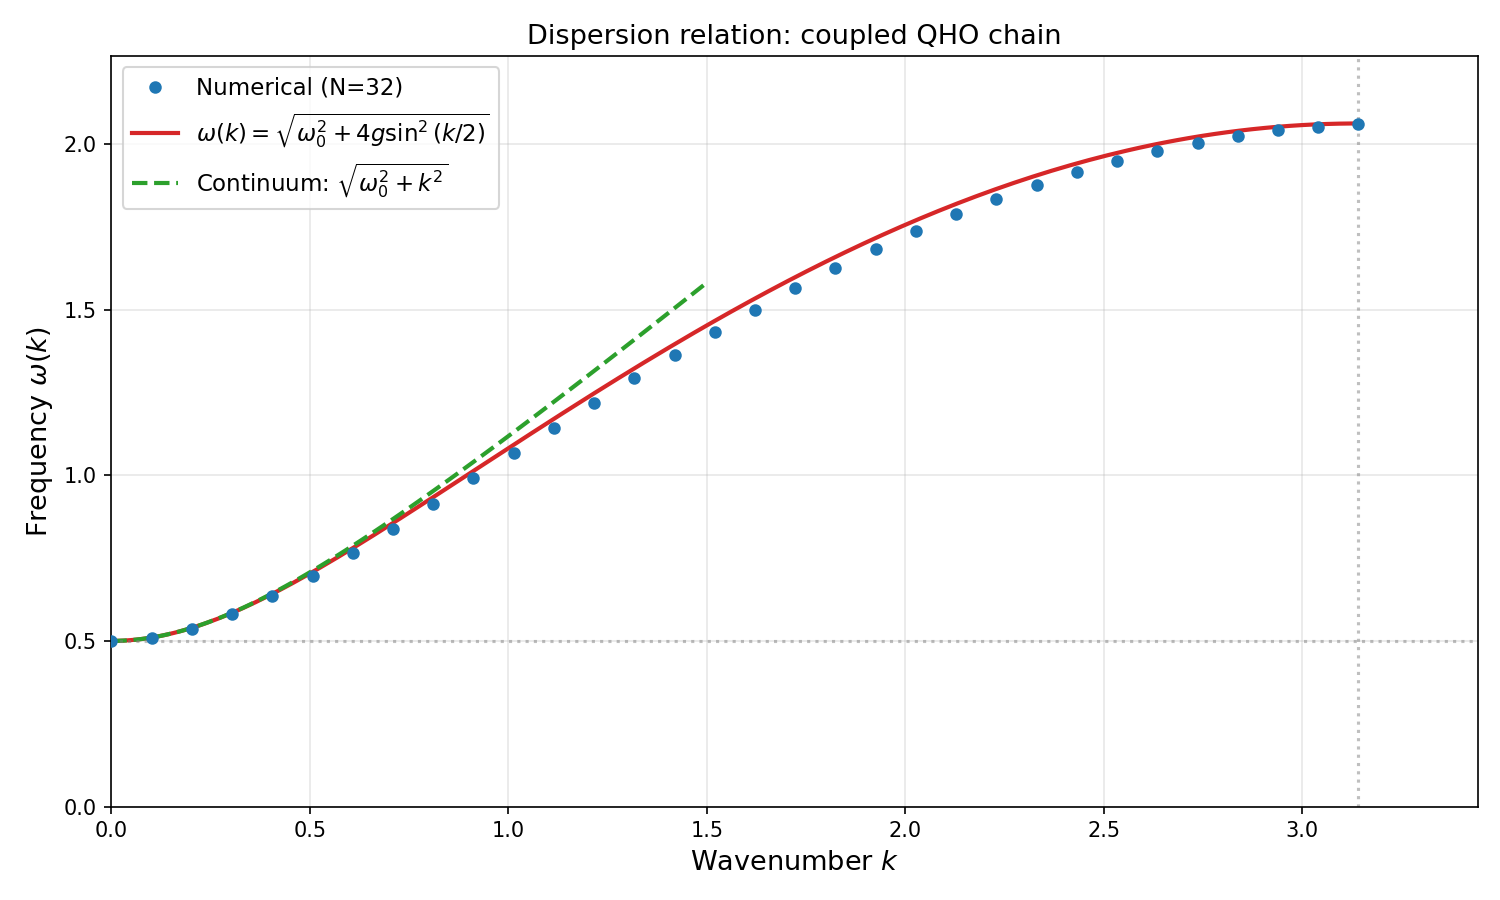
\includegraphics[width=0.8\textwidth]{04_dispersion.png}
\caption{耦合 QHO 链的色散关系。蓝色点为数值对角化结果，红色曲线为解析色散 $\omega(k) = \sqrt{\omega_0^2 + 4g\sin^2(k/2)}$，绿色虚线为连续极限 $\sqrt{\omega_0^2 + k^2}$。$k \ll 1$ 时三者一致。}
\label{fig:dispersion}
\end{figure}

图~\ref{fig:modes} 显示了前四个简正模式的振型。最低频的模式类似于长波振动，高频模式则有更多的节点结构。

\begin{figure}[htbp]
\centering
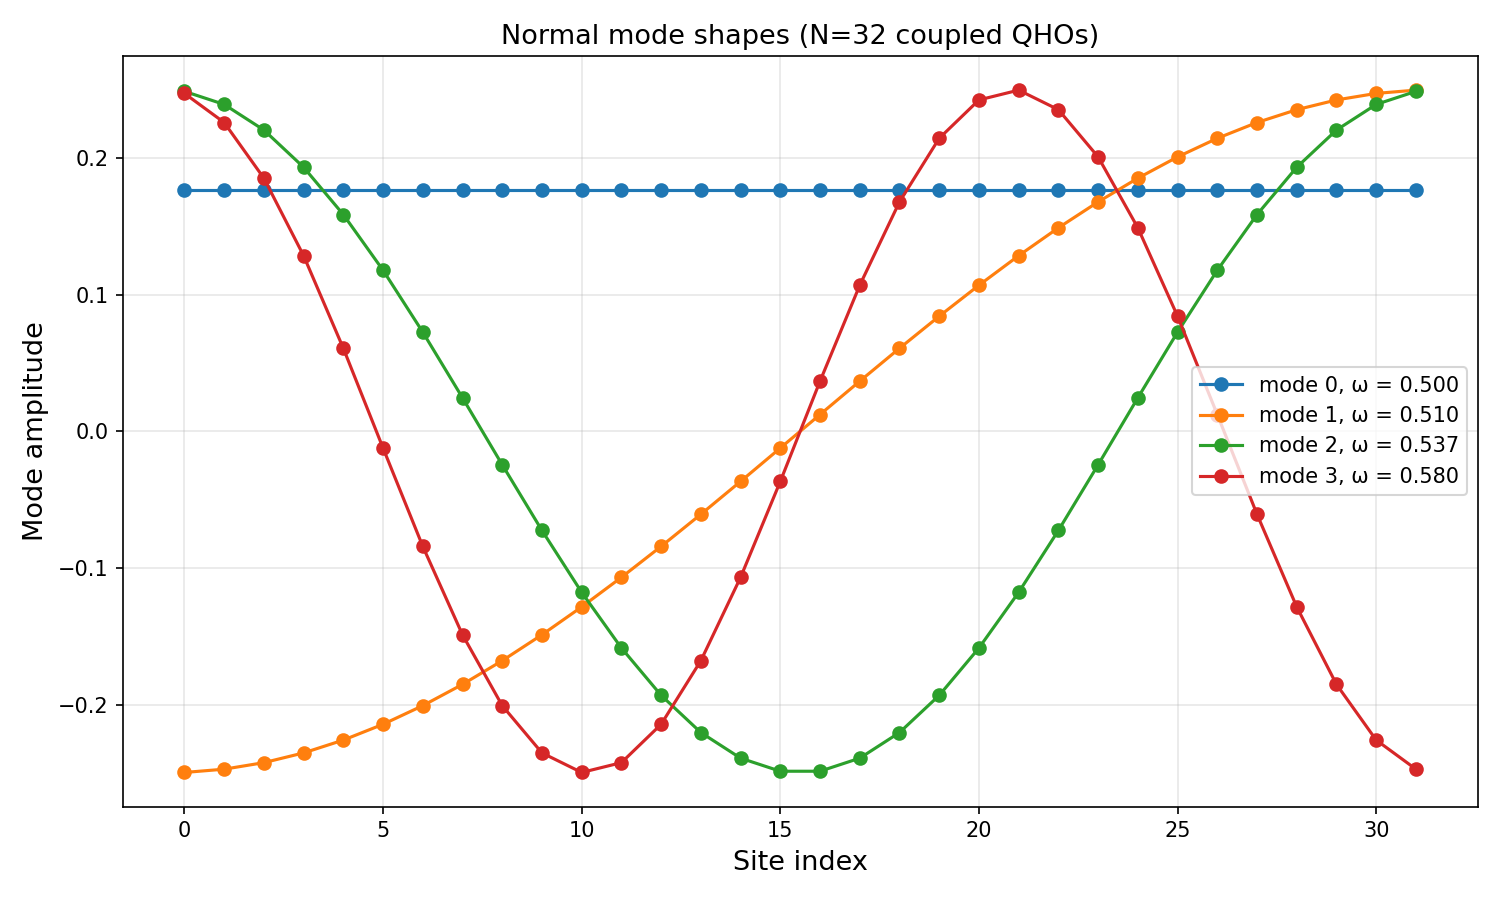
\includegraphics[width=0.8\textwidth]{04_normal_modes.png}
\caption{前四个简正模式的振型。频率最低的模式（蓝色）对应整链同向运动；频率较高的模式（绿色、红色、青色）有更多节点。这与弦振动或量子力学中的驻波完全类比。}
\label{fig:modes}
\end{figure}

\subsection{连续极限 → 场算符}

当 $N \to \infty$、晶格间距 $a \to 0$ 时，离散指标 $i$ 变为连续坐标 $x$，
而 $\hat x_i / \sqrt{a}$ 成为\textbf{场算符} $\hat\phi(x)$。

对应关系如下：
\begin{equation}
\begin{aligned}
\text{离散：}&\quad \hat x_i(t) \quad\text{在格点 $i$ 的振幅}\\
\text{连续：}&\quad \hat\phi(x, t) \quad\text{在时空点 $x$ 的场算符值}
\end{aligned}
\label{eq:continuum}
\end{equation}

对易关系从 $[\hat x_i, \hat p_j] = i\delta_{ij}$ 变为
\begin{equation}
[\hat\phi(t, \mathbf{x}), \hat\pi(t, \mathbf{y})] = i\delta^{(3)}(\mathbf{x} - \mathbf{y}).
\label{eq:field-comm}
\end{equation}

这里 $\hat\pi(t,\mathbf{x}) = \partial_t \hat\phi(t,\mathbf{x})$ 是与 $\hat\phi$ 共轭的动量密度。

\subsection{自由标量场的模式展开}

自由标量场 $\hat\phi(x)$ 在动量空间中可以写为：
\begin{equation}
\hat\phi(x) = \int \frac{d^3k}{(2\pi)^3} \frac{1}{\sqrt{2\omega_{\mathbf{k}}}}
\left( a_{\mathbf{k}} e^{-ikx} + a_{\mathbf{k}}^\dagger e^{ikx} \right),
\label{eq:field-expansion}
\end{equation}
其中 $\omega_{\mathbf{k}} = \sqrt{\mathbf{k}^2 + m^2}$，$kx = \omega_{\mathbf{k}}t - \mathbf{k}\cdot\mathbf{x}$。

产生湮灭算符满足
\begin{equation}
[a_{\mathbf{k}}, a_{\mathbf{k}'}^\dagger] = (2\pi)^3 \delta^{(3)}(\mathbf{k} - \mathbf{k}').
\label{eq:comm-continuum}
\end{equation}

\textbf{物理诠释：}
\begin{itemize}[nosep]
\item $a_{\mathbf{k}}^\dagger$ 在动量 $\mathbf{k}$ 处产生一个粒子，
相当于激发 $\mathbf{k}$ 谐振子模式到更高的 $n$ 态
\item $|0\rangle$ 是所有简正模式都处于基态的场——这就是\textbf{真空}
\item 单粒子态 $a_{\mathbf{k}}^\dagger |0\rangle$ 是场的某一种集体激发，
不是点粒子，而是弥散在整个空间的波包
\item 这里与 DMRG 的类比：Fock 空间 = $\bigotimes_k$（模式 $k$ 的 Fock 空间）
\end{itemize}

\section{从谐振子到场：三步走}

总结一下，从 QM 到 QFT 的思维跃迁分三步：

\begin{enumerate}[nosep]
\item \textbf{一个谐振子} $\to$ 一个粒子（$x$ 为坐标）
\item \textbf{多个耦合谐振子} $\to$ 多个简正模式（每个模式是独立的 QHO）
\item \textbf{连续极限} $\to$ 量子场（每个 $k$ 模式是独立 QHO）
\end{enumerate}

\begin{equation}
\begin{array}{c}
\text{连续梁振动} \\
\downarrow \\
\text{离散为耦合质量-弹簧} \\
\downarrow \\
\text{简正模式（独立 QHO）} \\
\downarrow \\
\text{量子化 → 声子}
\end{array}
\qquad\Longrightarrow\qquad
\begin{array}{c}
\text{自由标量场} \\
\downarrow \\
\text{格点离散化} \\
\downarrow \\
\text{动量模式（独立 QHO）} \\
\downarrow \\
\text{量子化 → 粒子（$\pi$/质子等）}
\end{array}
\label{eq:analogy-box}
\end{equation}

\begin{table}[htbp]
\centering
\caption{QHO 耦合链与自由场的一一对应}
\begin{tabular}{c|c}
\hline
耦合谐振子链 & 自由标量场 \\
\hline
$\hat x_i$（离散振幅） & $\hat\phi(x)$（场算符） \\
$\hat p_i$（离散动量） & $\hat\pi(x)$（动量密度） \\
$[\hat x_i, \hat p_j] = i\delta_{ij}$ & $[\hat\phi(x), \hat\pi(y)] = i\delta(x-y)$ \\
简正模式 $k$ & 动量模式 $\mathbf{k}$ \\
$\omega_k = \sqrt{\omega_0^2 + 4g\sin^2(k/2)}$ & $\omega_{\mathbf{k}} = \sqrt{\mathbf{k}^2 + m^2}$ \\
$a_k^\dagger$ 在模式 $k$ 产生声子 & $a_{\mathbf{k}}^\dagger$ 在动量 $\mathbf{k}$ 产生粒子 \\
\hline
\end{tabular}
\label{tab:analogy}
\end{table}

\section{真空不是空的}

真空 $|0\rangle$ 是所有简正模式都处于基态的态。
但谐振子的基态有零点能——它并不「空」。

在 QFT 中，$\hat\phi(x)$ 在真空中的期望值为零，但方差不为零：
\begin{equation}
\langle 0 | \hat\phi(x)^2 | 0 \rangle \neq 0.
\label{eq:vacuum-fluctuation}
\end{equation}
这意味着场在真空中不停地涨落——这就是\textbf{真空涨落}的起源。

你可以从耦合谐振子链直观理解：
即使链上每个质量都处于基态，连续极限下相邻点之间的关联函数 $\langle x_i x_j \rangle$ 不为零。
这对应着 QFT 中 $\langle 0 | \hat\phi(x)\hat\phi(y) | 0 \rangle \neq 0$——这就是\textbf{传播子}的起源。

\section{Phase 2：微扰论与 $\phi^4$ 相互作用}

前面我们处理的是自由场——所有模式独立、没有相互作用。
现在加上 $\phi^4$ 相互作用项，看看会发生什么。

\subsection{从单量子到场的相互作用}

在单量子层面，给谐振子加上非简谐项：
\begin{equation}
H = \underbrace{\frac12 p^2 + \frac12 \omega^2 x^2}_{H_0}
+ \underbrace{\lambda x^4}_{H_1},
\label{eq:anh-ham}
\end{equation}
其中 $\lambda x^4$ 就是「场的 $\phi^4$ 相互作用」在 $N=1$ 时的特例。

代码 \texttt{05\_anharmonic\_osc.py} 在 Fock 基矢中精确对角化这个 Hamiltonian，
并与微扰论（1 阶、2 阶 Rayleigh–Schrödinger）的结果比较。

\subsection{数值结果}

\begin{figure}[htbp]
\centering
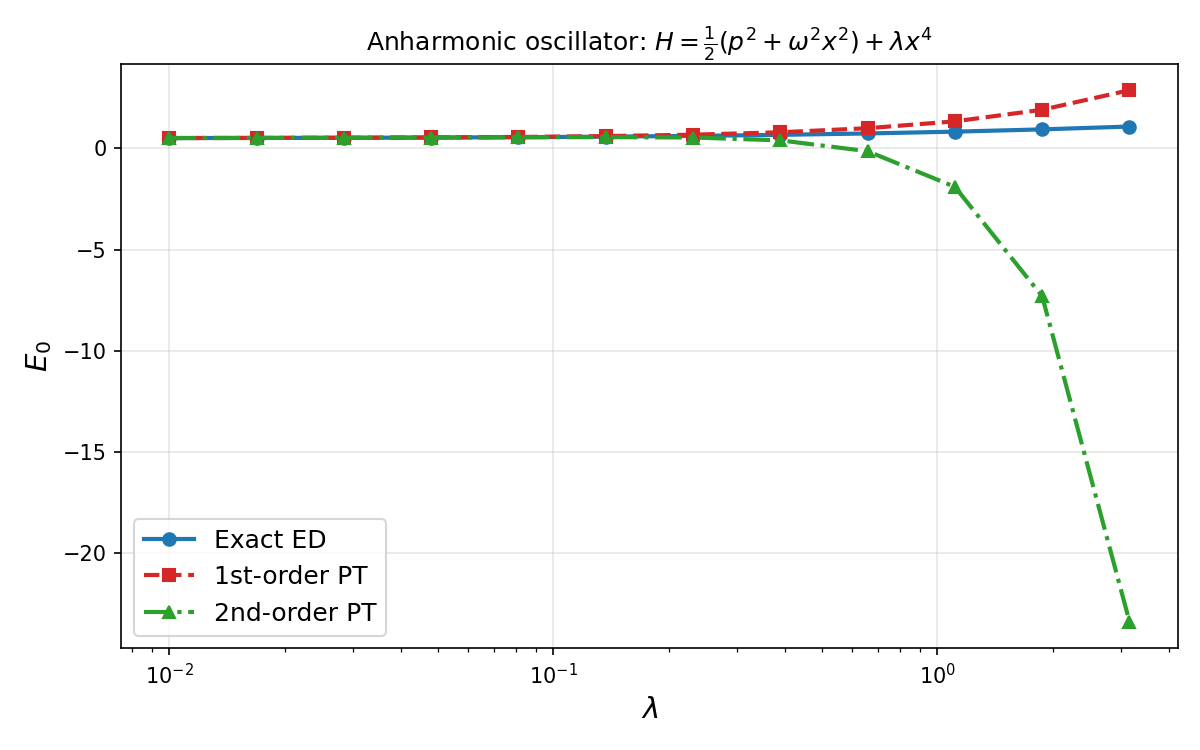
\includegraphics[width=0.8\textwidth]{05_anh_osc_E0.png}
\caption{非谐振子基态能量随 $\lambda$ 的变化。小 $\lambda$（$<0.1$）时 1 阶和 2 阶微扰都很好；
大 $\lambda$ 时微扰论发散，精确对角化仍然是可靠的。}
\label{fig:anh-e0}
\end{figure}

关键数字（$\lambda = 0.1$）：
\begin{itemize}[nosep]
\item 自由基态：$E_0^{(0)} = 0.5000$
\item 1 阶修正：$\langle 0| \lambda x^4 |0 \rangle = 0.0750$，$E_0^{(1)} = 0.5750$
\item 2 阶修正：$E_0^{(2)} = 0.5488$
\item 精确值：$E_0^{\text{exact}} = 0.5591$
\end{itemize}

\begin{figure}[htbp]
\centering
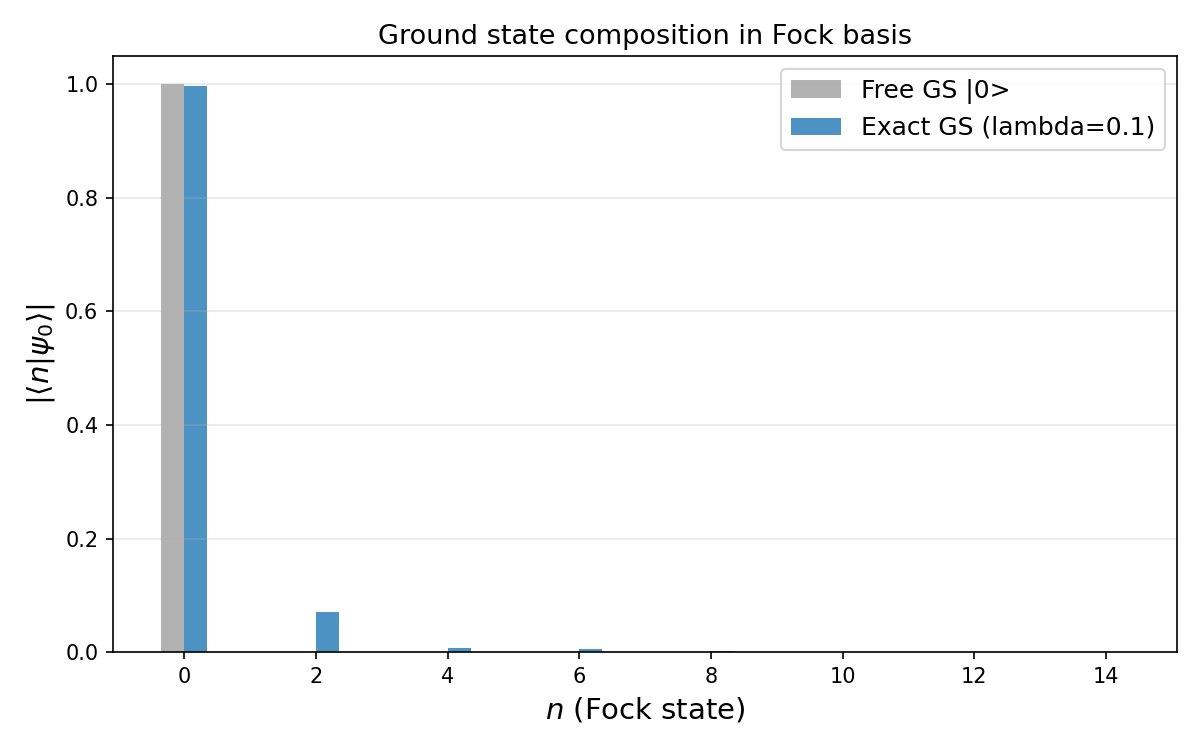
\includegraphics[width=0.8\textwidth]{05_anh_osc_wavefunction.png}
\caption{基态在 Fock 基矢中的组分。自由基态完全是 $|0\rangle$；
加上相互作用后 $|4\rangle$、$|8\rangle$ 等也有少量贡献（因为 $\lambda x^4$ 每次跃迁 $\Delta n = \pm 4$）。}
\label{fig:anh-wf}
\end{figure}

\subsection{tadpole 图的出场}

注意 1 阶修正 $\lambda\langle 0|x^4|0\rangle$ 的解析值：
\begin{equation}
\langle 0 | x^4 | 0 \rangle = \frac{3}{4\omega^2}.
\label{eq:tadpole-vacuum}
\end{equation}

在 $\phi^4$ 场论中，每个动量模式 $k$ 对应的谐振子都有类似的贡献。
全空间所有模式的总和给出真空能的单圈修正——这就是\textbf{tadpole 图}：
\begin{equation}
\Delta E_{\text{vac}} = \frac{\lambda}{4!} \times 3 \times
\int \frac{d^3k}{(2\pi)^3} \frac{1}{2\omega_{\mathbf{k}}}
\qquad\text{(对称因子}\ \frac12\text{)}.
\label{eq:tadpole-field}
\end{equation}

这正是我们在 Exercise 01（有限温）中算的 tadpole 在 $T=0$ 时的对应。
区别只在于：
\begin{itemize}[nosep]
\item $T=0$：真空期望值 $\dfrac{1}{2\omega_k}$（来自 $\langle 0|aa^\dagger|0\rangle$）
\item $T>0$：热期望值 $\dfrac{1}{2\omega_k} + \dfrac{n_B(\omega_k)}{\omega_k}$
\end{itemize}

\subsection{从代数到 Feynman 图：Wick 收缩}

$\langle 0| x^4 |0\rangle$ 可以用产生湮灭算符来算：
\begin{equation}
x^4 = \frac{1}{(2\omega)^2} (a + a^\dagger)^4.
\label{eq:x4-expand}
\end{equation}

展开后，只有完全配对的项（$a a^\dagger a a^\dagger$ 等）有非零真空期望值：
\begin{equation}
\langle 0| a a^\dagger a a^\dagger |0\rangle = 1\cdot 1 = 1,
\qquad
\langle 0| a a^\dagger a^\dagger a |0\rangle = 0,
\qquad\text{等}.
\label{eq:wick-example}
\end{equation}

所有非零配对的\textbf{个数}是 $3$（$C_3^1$ 种方式把两个 $a^\dagger$ 与两个 $a$ 配对）。
这就是 Wick 定理的雏形——它在 QFT 中对应 Feynman 图的收缩线。

\subsection{从单模式到场论}

把以上结果从 1 个谐振子推广到场论：
\[
\begin{array}{c}
N=1 \text{ 非谐振子} \\
\quad\quad\Big\downarrow \text{ 连续极限, 求和 } k \\
\phi^4 \text{ 场论：真空 tadpole}
\end{array}
\]

\begin{figure}[htbp]
\centering
\fbox{\parbox{0.5\textwidth}{
\begin{center}
$\displaystyle
\frac{\lambda}{2} \int \frac{d^3k}{(2\pi)^3} \frac{1}{2\omega_{\mathbf{k}}}
$
\end{center}
}}
\caption{$\phi^4$ 理论中的 tadpole 图。一根线自收缩形成回路——它代表的正是我们上面计算的 $\langle 0|x^4|0\rangle$ 的动量空间版本。}
\label{fig:tadpole-feynman}
\end{figure}

这样，一个从「单个非谐振子的微扰修正」出发的计算，最终落脚在「$\phi^4$ 场论的 Feynman 图」上。
这就是从 QM 走向 QFT 的具体路径。

\begin{enumerate}[nosep]
\item 算符场 $\hat\phi(x)$ 可以看作「每点一个谐振子」，相邻点的谐振子相互耦合
\item 动量空间使问题对角化：每个 $k$ 模式是独立谐振子
\item 粒子 = 场的量子化激发，对应某个 $k$ 模式的 $|0\rangle \to |1\rangle$ 跃迁
\item 真空有零点涨落 → 传播子 → 粒子可以在虚空中产生和湮灭
\item 你已有的 DMRG/MPS 直觉非常有帮助：QFT 的 Fock 空间 =\newline
$\bigotimes_{\mathbf{k}}$（模式 $\mathbf{k}$ 的 $\mathbb{C}^\infty$）的张量积空间
\end{enumerate}

\subsection{从单模式到格点：$\phi^4$ 场论的数值实现}

以上我们从单个非谐振子出发，得到了 tadpole 图的解析结果。
现在把它推广到 $N$ 个耦合谐振子——这\textbf{就是}格点 $\phi^4$ 场论。

在 $N$ 个格点的一维链上，Hamiltonian 为
\begin{equation}
H = \sum_{i=1}^N \left[\frac12 \pi_i^2 + \frac12 m^2 \phi_i^2\right]
+ \frac12 \sum_{i=1}^{N-1} (\phi_{i+1} - \phi_i)^2
+ \frac{\lambda}{4!} \sum_i \phi_i^4,
\label{eq:lat-ham}
\end{equation}
其中 $\pi_i$ 是与 $\phi_i$ 共轭的动量。

自由部分（$\lambda=0$）通过 Fourier 变换对角化，
得到 $N$ 个独立的简正模式，频率为
\begin{equation}
\omega_k^2 = m^2 + 4g\sin^2\frac{k}{2},
\qquad k = \frac{2\pi n}{N},\ n=0,1,\ldots,N-1.
\label{eq:lat-dispersion}
\end{equation}

相互作用项 $\lambda\phi_i^4/4!$ 耦合了这些模式。
其一阶基态能量修正为
\begin{equation}
\Delta E_0^{(1)} = \frac{\lambda}{4!} \sum_i \langle 0| \phi_i^4 |0\rangle.
\label{eq:lat-1st}
\end{equation}

由 Wick 定理，每个格点的四阶期望值分解为
\begin{equation}
\langle 0| \phi_i^4 |0\rangle = 3\, \bigl(\langle 0| \phi_i^2 |0\rangle\bigr)^2.
\label{eq:phi4-wick}
\end{equation}

而 $\langle 0| \phi_i^2 |0\rangle$ 通过模式展开计算：
\begin{equation}
\phi_i = \sum_k U_{ik} X_k,\qquad
X_k = \frac{1}{\sqrt{2\omega_k}} (a_k + a_k^\dagger),
\label{eq:mode-expansion}
\end{equation}
其中 $U_{ik}$ 是正交变换矩阵。由此得平移不变结果：
\begin{equation}
\langle 0| \phi_i^2 |0\rangle = \frac{1}{N} \sum_k \frac{1}{2\omega_k}.
\label{eq:phi2-vac}
\end{equation}

代入得解析 tadpole 求和：
\begin{equation}
\Delta E_0^{(1)} = \frac{\lambda}{24} N \cdot 3 \left(\frac{1}{N}\sum_k \frac{1}{2\omega_k}\right)^2
= \frac{\lambda}{8}\frac{1}{N}\left(\sum_k \frac{1}{2\omega_k}\right)^2.
\label{eq:tadpole-sum}
\end{equation}

代码 \texttt{06\_phi4\_lattice\_tadpole.py} 实现了上述计算的精确对角化验证。
它在每个模式 $k$ 的 Fock 空间中截断到 $N_{\text{fock}}$ 维，
通过张量积构造完整的 $N_{\text{fock}}^N$ 维 Hilbert 空间，
并显式构建 $\phi_i$ 算符和 $\phi_i^4$ 相互作用矩阵。

\begin{figure}[htbp]
\centering
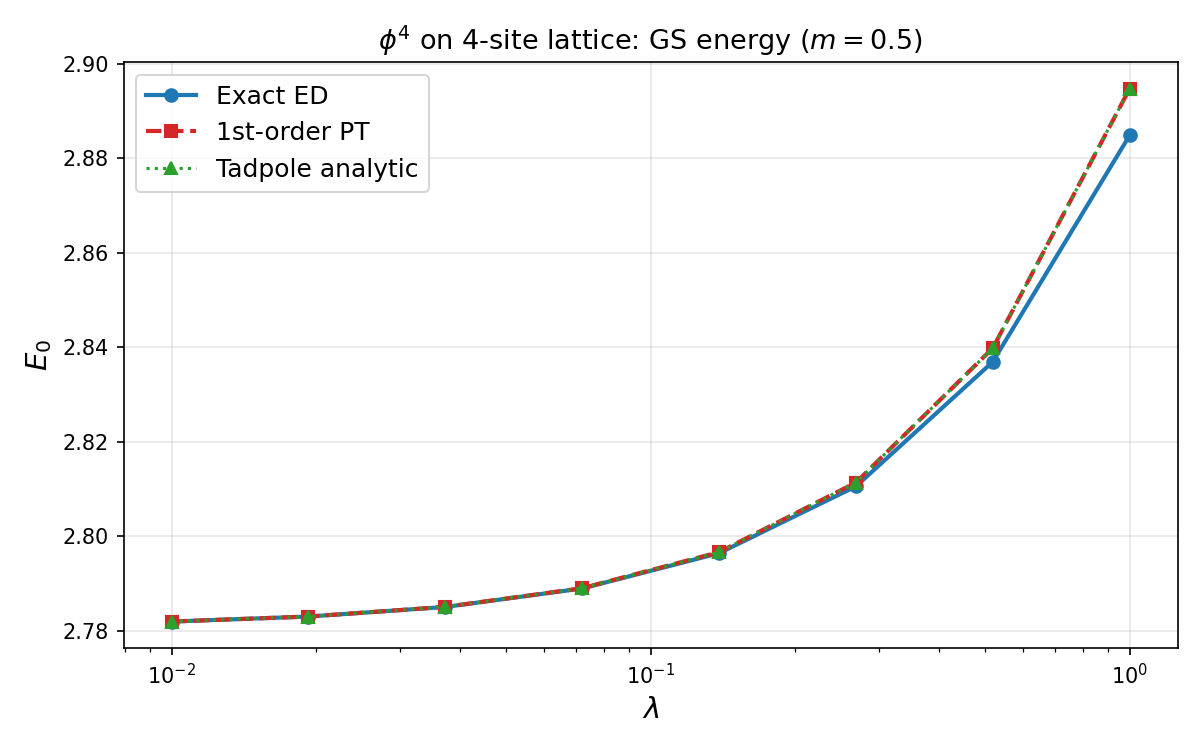
\includegraphics[width=0.8\textwidth]{06_phi4_lattice_E0.png}
\caption{格点 $\phi^4$ 基态能量随 $\lambda$ 的变化（$N=4$ 格点，$m=0.5$）。
精确对角化（蓝色实线）、一阶微扰（红色虚线）和 tadpole 解析公式（绿色点线）
在 $\lambda<0.1$ 时吻合很好。}
\label{fig:phi4-lattice}
\end{figure}

数值结果确认（$N=4$, $m=0.5$, $\lambda=0.05$）：
\begin{itemize}[nosep]
\item 自由基态能量：$E_0^{(0)} = 2.780776$
\item 一阶微扰修正：$\langle 0|H_1|0\rangle = 0.005695$
\item 解析 tadpole 公式与数值 $\langle 0|H_1|0\rangle$ 完全一致（误差 $2.6\times10^{-18}$）
\item 精确基态能量：$E_0 = 2.786442$，一阶微扰误差仅 $3\times10^{-5}$
\end{itemize}

$N\to\infty$ 连续极限下，模式求和变为动量积分：
\begin{equation}
\Delta E_0^{(1)} = \frac{\lambda}{8} \left[\int_{-\pi}^{\pi} \frac{dk}{2\pi} \frac{1}{2\omega_k}\right]^2.
\label{eq:continuum-tadpole}
\end{equation}

这正是在 Exercise 01（有限温 tadpole）中计算的 $T=0$ 版本。
唯一的区别是统计因子：
\begin{itemize}[nosep]
\item $T=0$：真空期望值 $\displaystyle\frac{1}{2\omega_k}$（来自 $\langle 0|aa^\dagger|0\rangle$）
\item $T>0$：热期望值 $\displaystyle\frac{1}{2\omega_k} + \frac{n_B(\omega_k)}{\omega_k}$
\end{itemize}

\vspace{1em}
\hrule
\vspace{0.5em}

从量子力学到场论的路径总结如下：

\begin{enumerate}[nosep]
\item 算符场 $\hat\phi(x)$ 可以看作「每点一个谐振子」，相邻点的谐振子相互耦合
\item 动量空间使问题对角化：每个 $k$ 模式是独立谐振子
\item 粒子 = 场的量子化激发，对应某个 $k$ 模式的 $|0\rangle \to |1\rangle$ 跃迁
\item 真空有零点涨落 → 传播子 → 粒子可以在虚空中产生和湮灭
\item 单谐振子的 $\lambda x^4$ 微扰修正 $\to$ $\phi^4$ 场论的 tadpole 图
\item 格点数值计算验证了从模式求和到 Feynman 图的完整对应
\item 你已有的 DMRG/MPS 直觉非常有帮助：QFT 的 Fock 空间 =\newline
$\bigotimes_{\mathbf{k}}$（模式 $\mathbf{k}$ 的 $\mathbb{C}^\infty$）的张量积空间
\end{enumerate}

\end{document}
